\section{Ampermetr va voltmetrga qo`shimcha qarshilik ulash}




\begin{enumerate}

\item Yuqori o‘lchash chegarasi $200$ mA bo‘lgan ampermetr yordamida $1000$ mA gacha bo‘lgan tok kuchini o‘lchash uchun qanday qarshilikli shuntdan foydalanish kerak ($\Omega$)? Ampermetrning qarshiligi $12~\Omega$.
\begin{enumerate}[label=\Alph*)]
\item 4
\item 5
\item 6
\item 3

\end{enumerate}

\item Ampermetrga parallel ulangan shuntning qarshiligi ampermetrning qarshiligidan $5$ marta kichik. Agar ampermetr $100$ mA tokni ko‘rsatayotgan bo‘lsa, magistraldagi tok kuchi $I$ qanday (mA) bo‘ladi?


\begin{enumerate}[label=\Alph*)]
\item 400
\item 500
\item 600
\item 800

\end{enumerate}

\item Shuntning qarshiligi $R$ ga, ampermetrning qarshiligi $4R$ ga teng. Agar magistraldagi tok kuchi $I=600$ mA bo‘lsa, ampermetr qanday tokni ko‘rsatadi (mA)?

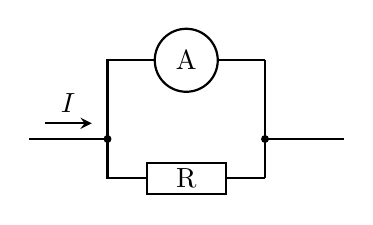
\begin{tikzpicture}[>=stealth, thick]
    % Asosiy kirish simi va tok yo'nalishi
    \draw (0,0) -- (1,0);
    \draw[->] (0.2,0.2) -- (0.8,0.2) node[midway, above] {$I$};

    % Tarmoqlanish nuqtasi (chapda)
    \draw (1,0) -- (1,1) -- (1.5,1); % Yuqoriga - ampermetrga
    \draw (1,0) -- (1,-0.5) -- (1.5,-0.5); % Pastga - shuntga

    % Ampermetr (yuqori tarmoq)
    \draw (2,1) circle (0.4) node {A};
    \draw (1.5,1) -- (1.6,1);
    \draw (2.4,1) -- (3,1);

    % Shunt qarshiligi (pastki tarmoq)
    \draw (1.5,-0.7) rectangle (2.5,-0.3) node[midway] {R};
    \draw (2.5,-0.5) -- (3,-0.5);

    % Birlashish nuqtasi (o'ngda)
    \draw (3,1) -- (3,-0.5);
    \draw (3,0) -- (4,0);
    \filldraw (1,0) circle (1pt);
    \filldraw (3,0) circle (1pt);

\end{tikzpicture}

\begin{enumerate}[label=\Alph*)]
\item 500
\item 120
\item 300
\item 200

\end{enumerate}

\item Ichki qarshiligi $180~\Omega$ bo‘lgan ampermetrning o‘lchash chegarasini $9$ marta oshirish uchun unga ulanadigan shuntning qarshiligi qanday bo‘lishi kerak ($\Omega$)?
\begin{enumerate}[label=\Alph*)]
\item 16,1
\item 18
\item 14
\item 22,5
\end{enumerate}

\item Ampermetrning ichki qarshiligi $12~\Omega$ bo‘lib, u $2,5$ A gacha tokni o‘lchashga mo‘ljallangan. Shu ampermetr bilan $15$ A gacha tokni o‘lchash uchun unga necha $\Omega$ li shunt ulash kerak?
\begin{enumerate}[label=\Alph*)]
\item 3,1
\item 1,1
\item 2,4
\item 4,2

\end{enumerate}

\item Zanjirga ulangan ampermetrning ichki qarshiligi $11~\Omega$ va shuntning qarshiligi $2,2~\Omega$. Ampermetr $13$ A tokni ko‘rsatsa, zanjirdagi tok kuchi necha Amperga teng bo‘ladi?
\begin{enumerate}[label=\Alph*)]
\item 78
\item 66
\item 20
\item 82
\end{enumerate}

\item Ikkita bir xil shuntlardan iborat ampermetrga ulansa, uning bo‘lim qiymati $3$ marta ortadi. Agar ikkala shunt ampermetrga parallel ulansa, uning o‘lchash chegarasi necha marta ortadi?
\begin{enumerate}[label=\Alph*)]
\item 3
\item 4
\item 5
\item 2,5
\end{enumerate}

\item Ikkita bir xil shunt o‘zaro ketma-ket ulanib, so‘ngra ampermetrga ulansa, uning o‘lchash chegarasi $4,5$ marta ortadi. Ikkala shunt ampermetrga parallel ulanganida ampermetrning o‘lchash chegarasi necha marta ortadi?
\begin{enumerate}[label=\Alph*)]
\item 6,5
\item 9
\item 15
\item 18
\end{enumerate}

\item Qarshiligi $0,04~\Omega$ bo‘lgan ampermetrga uzunligi $15$ cm va ko‘ndalang kesim yuzi $3$ mm$^2$ bo‘lgan mis sim parallel ulangan. Ampermetr $0,17$ A tokni ko‘rsatadi. Simdagi tok kuchini toping (A). Misning solishtirma qarshiligi $1,7\cdot10^{-8}~\Omega\cdot$m.
\begin{enumerate}[label=\Alph*)]
\item 2,8
\item 4
\item 5
\item 8
\end{enumerate}

\item Voltmetrning ichki qarshiligi $300~\Omega$. Unga $1200~\Omega$ qo‘shimcha qarshilik ulansa, shkala bo‘lim qiymati necha marta o‘zgaradi?
\begin{enumerate}[label=\Alph*)]
\item 3
\item 4
\item 5
\item 6
\end{enumerate}

\item Voltmetrning ichki qarshiligi $2$ k$\Omega$ bo‘lib, u $8$ V ni o‘lchashga mo‘ljallangan. Shu voltmetrga qanday qo‘shimcha qarshilik (k$\Omega$) ulanganda, u bilan $40$ V kuchlanishni o‘lchash mumkin bo‘ladi?
\begin{enumerate}[label=\Alph*)]
\item 5
\item 12
\item 18
\item 8
\end{enumerate}

\item Qarshiligi $1600~\Omega$ bo‘lgan voltmetr $15$ V gacha kuchlanishni o‘lchashga mo‘ljallangan. Shu voltmetr bilan $210$ V gacha kuchlanishni o‘lchash uchun unga qanday qo‘shimcha qarshilik ulash kerak ($\Omega$)?
\begin{enumerate}[label=\Alph*)]
\item 150
\item 20,8
\item 30
\item 27
\end{enumerate}

\item $15$ V kuchlanishni o‘lchashga mo‘ljallangan voltmetr bilan $270$ V kuchlanishni o‘lchash uchun unga qanday qarshilik ulash kerak ($\Omega$)? Voltmetrning qarshiligi $300~\Omega$ ga teng.
\begin{enumerate}[label=\Alph*)]
\item 5400
\item 5500
\item 5600
\item 5100
\end{enumerate}

\item $20$ V kuchlanishni o‘lchashga mo‘ljallangan voltmetr bilan $150$ V kuchlanishni o‘lchash uchun unga qanday qo‘shimcha qarshilik ($\Omega$) ulash kerak? $R_v=200~\Omega$.
\begin{enumerate}[label=\Alph*)]
\item 1300
\item 1500
\item 1400
\item 1600
\end{enumerate}

\item Ichki qarshiligi $2800~\Omega$ bo‘lgan voltmetr elektr tarmog‘iga ulanganda, $120$ V kuchlanishni ko‘rsatdi. Voltmetrga necha $\Omega$ qarshilik ketma-ket ulansa, u $80$ V ni ko‘rsatadi?
\begin{enumerate}[label=\Alph*)]
\item 2700
\item 1700
\item 2100
\item 1400
\end{enumerate}

\item Sxemada $R_1=800~\Omega$, $R_2=1000~\Omega$ va shu zanjirning umumiy qarshiligi $480~\Omega$ bo‘lsa, voltmetrning o‘lchash chegarasi necha marta oshirilgan?

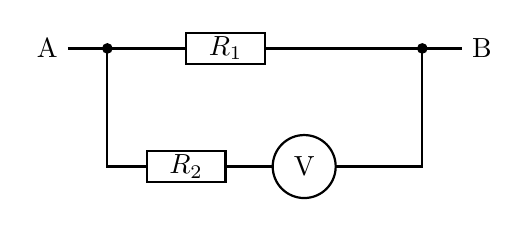
\begin{tikzpicture}[>=stealth, thick]
    % Asosiy tarmoq va A, B nuqtalari
    \draw (0,0) node[left] {A} -- (0.5,0);
    \draw (4.5,0) -- (5,0) node[right] {B};

    % Yuqori tarmoq (R1 qarshilik bilan)
    \draw (0.5,0) -- (1.5,0);
    \draw (1.5,-0.2) rectangle (2.5,0.2) node[midway] {$R_1$};
    \draw (2.5,0) -- (4.5,0);

    % Pastki tarmoq (R2 qarshilik va V voltmetr bilan)
    \draw (0.5,0) -- (0.5,-1.5) -- (1,-1.5);
    \draw (1,-1.7) rectangle (2,-1.3) node[midway] {$R_2$};
    \draw (2,-1.5) -- (2.6,-1.5);
    \draw (3,-1.5) circle (0.4) node {V};
    \draw (3.4,-1.5) -- (4.5,-1.5) -- (4.5,0);

    % Tugun nuqtalarini belgilash
    \filldraw (0.5,0) circle (1.5pt);
    \filldraw (4.5,0) circle (1.5pt);

\end{tikzpicture}

\begin{enumerate}[label=\Alph*)]
\item 3
\item 4
\item 5
\item 6
\end{enumerate}

\end{enumerate}

\begin{table}[!ht]
\centering
\begin{tabular}{|c|c|c|c|c|c|c|c|c|c|}
\hline
1d & 2c & 3b & 4d & 5c & 6a & 7c & 8c & 9d & 10c \\ \hline
11d & 12b & 13d & 14a & 15d & 16d &  &  &  &  \\ \hline
\end{tabular}
\end{table}
